%%%%%%%%%%%%%%%%%%%%%%%%%%%%%%%%%%%%%%%%%%%%%%%%%%%%%%%%%%%%%%%%%%%%%%%%%%%%%
%
%  System        : 
%  Module        : 
%  Object Name   : $RCSfile$
%  Revision      : $Revision$
%  Date          : $Date$
%  Author        : $Author$
%  Created By    : Robert Heller
%  Created       : Fri May 3 11:25:06 2024
%  Last Modified : <240503.2324>
%
%  Description 
%
%  Notes
%
%  History
% 
%%%%%%%%%%%%%%%%%%%%%%%%%%%%%%%%%%%%%%%%%%%%%%%%%%%%%%%%%%%%%%%%%%%%%%%%%%%%%
%
%    Copyright (C) 2024  Robert Heller D/B/A Deepwoods Software
%			51 Locke Hill Road
%			Wendell, MA 01379-9728
%
%    This program is free software; you can redistribute it and/or modify
%    it under the terms of the GNU General Public License as published by
%    the Free Software Foundation; either version 2 of the License, or
%    (at your option) any later version.
%
%    This program is distributed in the hope that it will be useful,
%    but WITHOUT ANY WARRANTY; without even the implied warranty of
%    MERCHANTABILITY or FITNESS FOR A PARTICULAR PURPOSE.  See the
%    GNU General Public License for more details.
%
%    You should have received a copy of the GNU General Public License
%    along with this program; if not, write to the Free Software
%    Foundation, Inc., 675 Mass Ave, Cambridge, MA 02139, USA.
%
% 
%
%%%%%%%%%%%%%%%%%%%%%%%%%%%%%%%%%%%%%%%%%%%%%%%%%%%%%%%%%%%%%%%%%%%%%%%%%%%%%

\documentclass[12pt,twoside,letterpaper]{article}
\usepackage{graphicx}
\usepackage{mathptm}
\usepackage{times}
\usepackage{makeidx}
\usepackage{ifpdf}
\usepackage{footmisc}
\ifpdf
\usepackage[pdftex,
            pagebackref=true,
            colorlinks=true,
            linkcolor=blue,
            unicode
           ]{hyperref}
\else
\usepackage[ps2pdf,
            pagebackref=true,
            colorlinks=true,
            linkcolor=blue,
            unicode
           ]{hyperref}
\usepackage{pspicture}
\fi
\usepackage{url}
\pagestyle{headings}
\emergencystretch=50pt
\setcounter{tocdepth}{3}
\setcounter{secnumdepth}{3}
\title{FRED (EOT) flashing board.}
\author{Robert Heller \\ The Country Robot \\ Wendell, MA, USA}
\date{\today}
\begin{document}
\maketitle

This is a circuit board that implements a FRED (Flashing Rear End 
Device)\footnote{Also know as an EOT (End Of Train) device.}. This little 
circuit board rides in the trailing truck of the last freight car of a train 
and flashes a LED mounted on a FRED riding in the trailing coupler of that 
freight car.

\section{Assembly}


\section{Separating the two boards}
\begin{figure}[hbpt]\begin{centering}%
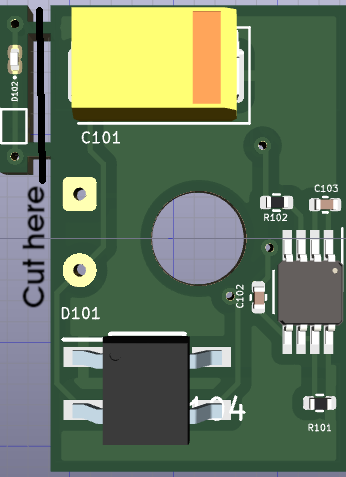
\includegraphics[width=3in]{FRED_Board3D_Top_cut.png}
\caption{Cutting the boards apart}
\label{fig:boardcut}
\end{centering}\end{figure}
The circuit board is mostly assembled.  It is necessary to solder on two small 
pieces of phosphor bronze that will be the wiper contacts to pick up power 
from the track. The two small pieces of phosphor bronze are soldered onto the 
labeled pad on the back side of the board and then bent into ``V'' shapes. It 
is also necessary to cut the board into two pieces, as shown in 
Figure~\ref{fig:boardcut}. After cutting the boards apart, carefully sand the 
cuts flush.

\section{Installing the power pickup wipers on the main board}

\begin{figure}[hbpt]\begin{centering}%
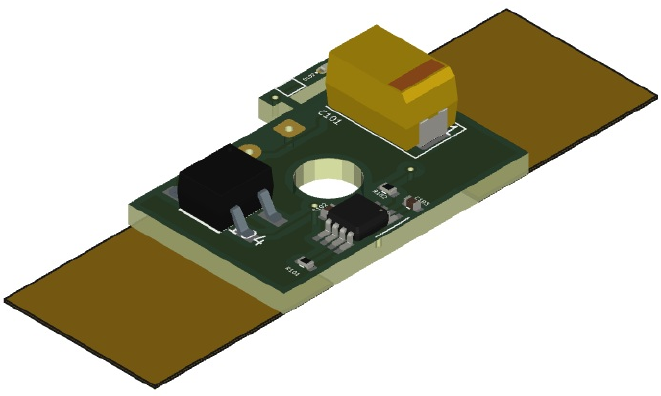
\includegraphics[width=3in]{FRED_with_wipers_not_bent.png}
\caption{Wiper strips soldered on}
\label{fig:FRED_with_wipers_not_bent}
\end{centering}\end{figure}
\begin{figure}[hbpt]\begin{centering}%
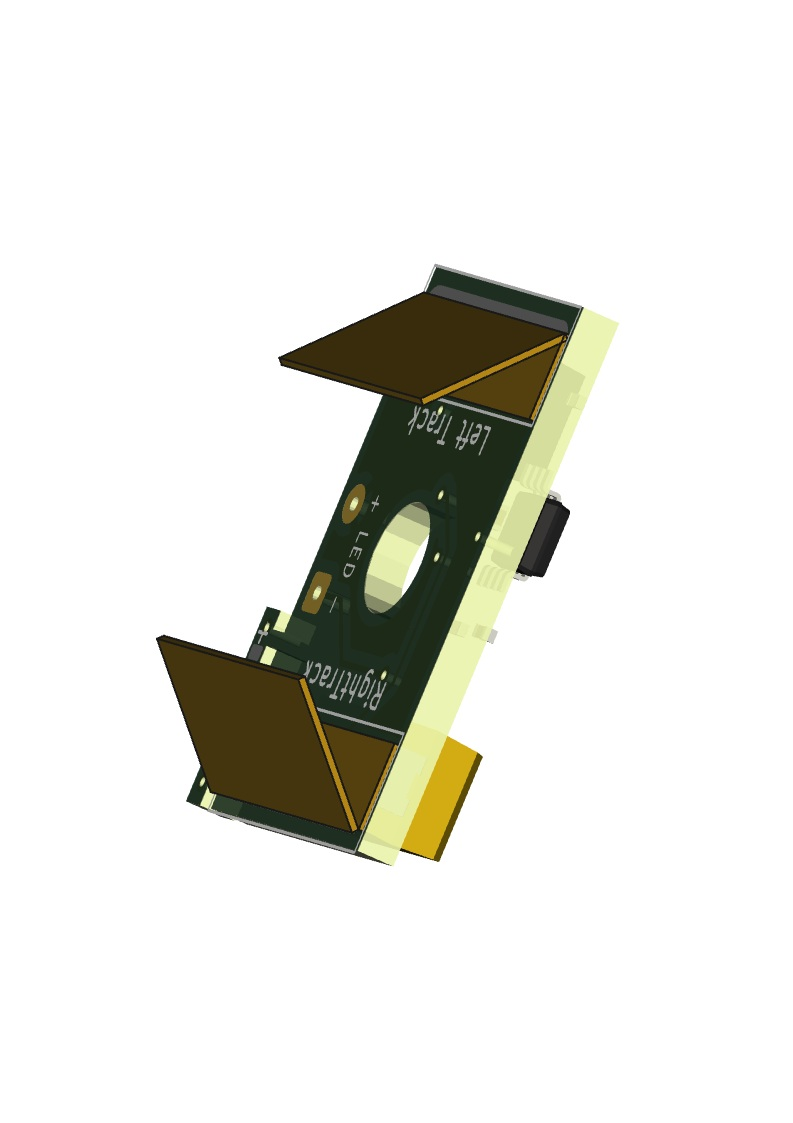
\includegraphics[width=3in]{FRED_with_wipers_bent.png}
\caption{Wiper strips bent}
\label{fig:FRED_with_wipers_bent}
\end{centering}\end{figure}
Next cut two pieces of phosphor bronze sheet, 13.5mm x 16mm and solder them to
the pads on the bottom at the ends of the nain board, with 12.5mm extending
beyond the ends of the board, as shown in
Figure~\ref{fig:FRED_with_wipers_not_bent}. Once soldered, bend the pieces up
(under the board) as shown in Figure~\ref{fig:FRED_with_wipers_bent}.

\section{Installing the LED board on the EOT}

If you model EOT does not have a LED in it you can use the little LED board. 
You can sand down the back of the EOT and drill a hole for the LED on the LED 
board.  Then glue the LED board on the back of the EOT, with the LED in the 
hole.

\section{Wiring}

Solder two fine gauge hookup wires (typically red on plus(+) and black on 
negative(-)) between the EOT's LED (or LED board) and the back side of the 
main board.  The wires need to be long enough to reach from the coupler and 
the truck, with a little extra to allow for truck movement.

\section{Installing on a car}

You need a car with metal wheels and metal axles (which have an insulator on 
one wheel).  Pop one wheelset out and hook one of the wipers on the remaining 
wheelset axle.  Fit the removed wheelset in the other wiper, taking care that 
the insulator is at the opposite side from the wheelset.  Pop the wheelset in 
place.  The board should now be suspended from the wipers hanging on the 
axles. 









\end{document}
